\chapter{A Mecânica dos Sólidos: tensão, deformação e deslocamento}

A Mecânica dos Sólidos estuda o comportamento de objetos sólidos sob carregamentos externos, aplicando métodos analíticos para determinar características de resistência, rigidez e estabilidade. Sua aplicação é voltada ao projeto de estruturas a fim de que cumpram determinadas exigências, tais como deformação máxima, capacidade de carga e peso, ou economia de materiais. E, por meio de ferramentas matemáticas, estuda os efeitos de tensão e deformação no interior de corpos sólidos \cite[pág. 2]{popov}.


Um corpo sólido por ser descrito como um conjunto de pontos materiais que resistem a forças cisalhantes, ou seja, que resistem a trações tangenciais às suas superfícies. Neste trabalho são considerados corpos sólidos elásticos, homogêneos e isotrópicos. Aqui, um corpo com essas características é denominado $\mathcal{B}$.

Corpos sólidos elásticos são aqueles que, quando submetidos a carregamentos, deformam-se, mas quando o carregamento é retirado, retornam à sua forma original. Corpos sólidos homogêneos são aqueles que possuem as mesmas propriedades físicas em todos os pontos materiais (tais como massa específica, rigidez etc.), de modo que uma porção do corpo seja indistinta do restante. Corpos sólidos isotrópicos são aqueles que possuem as mesmas propriedades físicas em todas as direções do espaço.

Este capítulo aborda os seguintes temas de Mecânica dos Sólidos, relevantes para o desenvolvimento inicial do módulo PHILLIPO.jl voltado à análise de estruturas elásticas sob carregamentos constantes:
\begin{enumerate}
    \item conceito de tensão;
    \item conceito de deslocamento e deformação;
    \item comportamento dos materiais: a lei de Hooke generalizada;
\end{enumerate}

\section{Tensão}

Um corpo sólido se deforma quando submetido a carregamentos externos\footnote{Expressão que se refere tanto a carregamentos térmicos, quanto mecânicos, embora o primeiro não seja assunto deste texto.} sobre sua geometria, de modo que qualquer seção plana arbitrária do corpo revele forças internas que estejam em equilíbrio entre si, e que sejam balanceadas pelos carregamentos externos. As forças internas geralmente variam ao longo do corpo, como também dependem da orientação do plano dessa seção. 
Seja um corpo $\mathcal{B}$, sólido, em equilíbrio e de geometria qualquer, descrito sobre um sistema de referência ($xyz$ com origem em $o$), submetido a forças externas na forma do carregamento $\bm{F}$ (veja figura \ref{fig:forcas_internas}). Sejam também as seções $S_{1,2,3}$, planos de corte através desse corpo (normais aos versores do sistema de referência), em que atuam as forças internas $\bm{P}$, conforme a figura \ref{fig:forcas_internas_2}. $\Delta \bm{P}$ é a resultante de forças que atuam sobre uma área $\Delta A$ (centrada em um certo ponto $p$), pertencente a $S$. O limite da razão entre cada componente de $\Delta \bm{P}$ (tangenciais e normais) e a área $\Delta A$, quando $\Delta A \to 0$, define o vetor tração, cuja decomposição nos eixos $x$, $y$ e $z$, define as componentes do tensor tensão sobre o ponto $p$, de forma que
\begin{equation}
    \tau_{xx} = \lim_{\Delta A_x \to 0} \frac{\Delta P_x}{\Delta A_x}, \qquad
    \tau_{xy} = \lim_{\Delta A_x \to 0} \frac{\Delta P_y}{\Delta A_x}, \qquad
    \tau_{xz} = \lim_{\Delta A_x \to 0} \frac{\Delta P_z}{\Delta A_x},
\end{equation}
em que os índices de $\tau$ indicam, o primeiro, a normal do plano infinitesimal em que a tensão atua, e, o segundo, sua direção. Por conveniência, as tensões normais (aquelas que atuam perpendicularmente ao plano) são representadas por $\sigma$, ao invés de se utilizar $\tau$ com índices repetidos ($\tau_{xx} \equiv \sigma_x$). O símbolo $\tau$, então, é reservado às tensões de cisalhamento, que atuam tangencialmente ao plano infinitesimal. No SI, a tensão é mensurada em Pascal ([Pa] = [N/m²]) \cite[pág. 5]{popov}.

\begin{figure}
    \centering
    \caption{Forças internas: seção em um sólido qualquer}
    \begin{subfigure}[b]{\textwidth}
        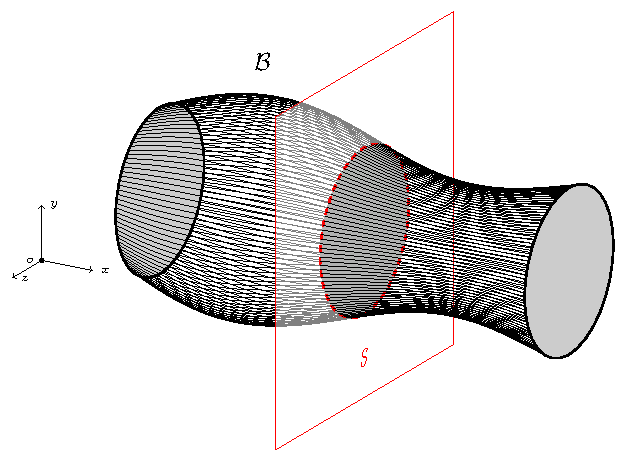
\includegraphics[scale=0.7]{Figuras/forcas_internas_2.pdf}
        \caption{$ $}
        \label{fig:forcas_internas_1}
    \end{subfigure}
    \hfill
    \begin{subfigure}[b]{\textwidth}
        \centering
        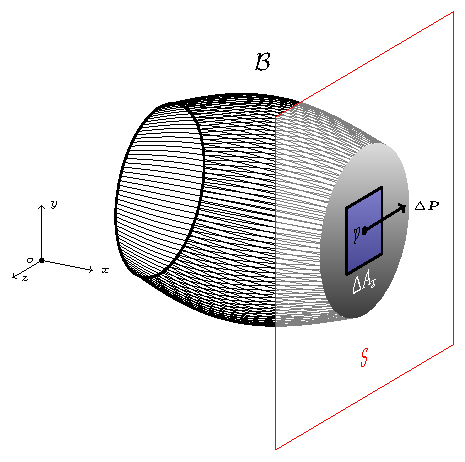
\includegraphics[scale=0.7]{Figuras/forcas_internas_1.pdf}
        \caption{$ $}
        \label{fig:forcas_internas_2}
    \end{subfigure}
    \hfill
    \begin{subfigure}[b]{\textwidth}
        \centering
        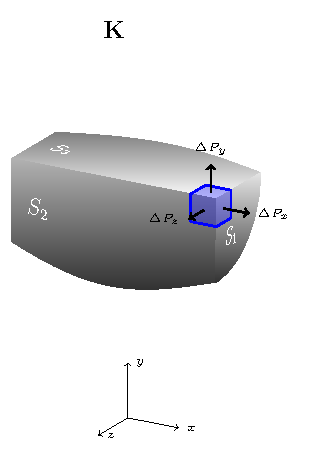
\includegraphics[scale=0.7]{Figuras/forcas_internas_3.pdf}
        \caption{$ $}
        \label{fig:forcas_internas_3}
    \end{subfigure}
       \label{fig:forcas_internas}
\end{figure}

Se o mesmo procedimento for realizado para cada face do elemento cúbico, formado por mais três seções paralelas a $S_{1,2,3}$ da figura \ref{fig:forcas_internas_3}, teremos a configuração da tração em três planos perpendiculares entre si para um certo ponto $p$ em $\mathcal{B}$,  conforme a figura \ref{fig:estado_de_tensao}, o que descreve o estado de tensão para aquele ponto. As componentes do estado de tensão podem ser dispostas na forma de uma matriz representativa do tensor de segunda ordem, denominado tensor de tensões, e, de acordo com \citeshort{popov}, é

\begin{equation}
    \bm{\sigma} =
    \begin{bmatrix}
        \sigma_x & \tau_{yx} & \tau_{zx} \\
        \tau_{xy} & \sigma_{y} & \tau_{zy} \\
        \tau_{xz} & \tau_{yz} & \sigma_{z} \\
    \end{bmatrix},
\end{equation}
em que a linha indica o plano em que a componente age, e a coluna, sua direção.

O tensor de tensões é simétrico, o que pode ser demonstrado realizando o somatório de momentos sobre o elemento infinitesimal de tensão, de modo que esteja em equilíbrio. Oportunamente, escolhendo o ponto central para a análise do equilíbrio angular, podemos descrever as seguintes relações \cite[pág. 8]{popov}:

\begin{equation}
    \begin{cases}
        \displaystyle  \vec{i} : \tau_{zy} (dxdy) \frac{dz}{2} - \tau_{yz} (dx dz) \frac{dy}{2} - \tau_{zy} (dydx) \frac{dz}{2}+ \tau_{yz} (dxdy) \frac{dy}{2} = 0 \\

        \displaystyle  \vec{j} : \tau_{xz} (dydz) \frac{dx}{2} - \tau_{zx} (dx dy) \frac{dz}{2} - \tau_{zx} (dx dy) \frac{dz}{2} + \tau_{xz} (dydz) \frac{dx}{2} = 0 \\

        
        \displaystyle  \vec{k} : \tau_{yx} (dxdz) \frac{dy}{2} - \tau_{xy} (dydz) \frac{dx}{2} - \tau_{xy} (dydz) \frac{dx}{2} + \tau_{yx} (dxdz) \frac{dy}{2} = 0 \\

    \end{cases} \implies
    \begin{cases}
        \tau_{zy} = \tau_{yz} \\
        \tau_{xz} = \tau_{zx} \\
        \tau_{yx} = \tau_{xy} \\
    \end{cases}.
\end{equation}
Portanto,
\begin{equation}
    \tau_{ij} = \tau_{ji} \iff \bm{\sigma} = \bm{\sigma}^t.
\end{equation}
Essa propriedade implica que o tensor de tensões possua apenas seis componentes independentes, ao invés de nove. Aproveitando-se disso, a notação de Voigt distribui as componentes independentes em uma matriz coluna de seis elementos, tal que, de acordo com \citeshort{roylance},

\begin{equation}
    \{\bm{\sigma}\} = \begin{bmatrix}
        \sigma_x & \sigma_y & \sigma_z & \tau_{xy} & \tau_{xz} & \tau_{yz}
    \end{bmatrix}^t.
\end{equation}


\begin{figure}
    \centering
    \caption{Estado de tensão}
    \begin{tikzpicture}[3d view = {-60}{-20}, scale=2]
        \draw[->] (0,0,0) --++ (3,0,0) node[right]{$x$};
        \draw[->] (0,0,0) --++ (0,3,0) node[left]{$y$};
        \draw[->] (0,0,0) --++ (0,0,3) node[above]{$z$};
        
        \draw[very thick, blue] (0,0,0) --++ (2,0,0) --++ (0,0,2)--++ (-2,0,0) -- cycle;
        \draw[very thick, blue] (0,2,0) --++ (2,0,0) --++ (0,0,2)--++ (-2,0,0) -- cycle;
        \draw[very thick, blue] (0,0,0) --++ (0,2,0) --++ (0,0,2) --++ (0,-2,0) -- cycle;
        \draw[very thick, blue] (2,0,0) --++ (0,2,0) --++ (0,0,2) --++ (0,-2,0) -- cycle;
        \draw[line width=1mm, blue, fill = blue, fill opacity = 0.5] (2,0,0) --++ (0,0,2) --++ (-2,0,0) --++ (0,2,0) --++ (0,0,-2) --+(2,0,0) -- cycle;
        
        
        \draw[arrows = {-Latex[width=10pt, length=10pt]},very thick, line width = 1mm] (2,1,1) --++ (1,0,0) node[right]{$\sigma_x$};
        \draw[arrows = {-Latex[width=10pt, length=10pt]},very thick, line width = 1mm] (1,2,1) --++ (0,1,0) node[left]{$\sigma_y$};
        \draw[arrows = {-Latex[width=10pt, length=10pt]},very thick, line width = 1mm] (1,1,2) --++ (0,0,1) node[right]{$\sigma_z$};
        
        \draw[arrows = {-Stealth[harpoon,swap]} ,very thick, line width = 1mm] (2,1,0.1) --++ (0,0,1.8) node[right]{$\tau_{xz}$};
        \draw[arrows = {-Stealth[harpoon]} ,very thick, line width = 1mm] (2,0.1,1) --++ (0,1.7,0) node[above]{$\tau_{xy}$};

        \draw[arrows = {-Stealth[harpoon]} ,very thick, line width = 1mm] (1,2,0.1) --++ (0,0,1.8) node[left]{$\tau_{yz}$};
        \draw[arrows = {-Stealth[harpoon,swap]} ,very thick, line width = 1mm] (0.1,2,1) --++ (1.7,0,0) node[below]{$\tau_{yx}$};               
        
        \draw[arrows = {-Stealth[harpoon]} ,very thick, line width = 1mm] (0.1,1,2) --++ (1.8,0,0) node[left]{$\tau_{zx}$};
        \draw[arrows = {-Stealth[harpoon,swap]} ,very thick, line width = 1mm] (1,0.1,2) --++ (0,1.8,0) node[above]{$\tau_{zy}$};        
        
        
    \end{tikzpicture}
    \label{fig:estado_de_tensao}
\end{figure}

\subsection{Equações diferenciais governantes do equilíbrio estático}

Outro fato importante sobre o estado de tensão vem do equilíbrio de forças. Assumindo que a distribuição de tensão $\bm{\sigma}(x,y,z)$ é contínua e diferenciável ao longo do domínio $\Omega$ do sólido $\mathcal{B}$, podemos analisar sua variação sobre um elemento cúbico infinitesimal, de modo que a força resultante sobre ele seja nula. Como o tensor de tensões representa a decomposição das forças internas agindo sobre as faces de um cubo infinitesimal, o somatório de forças é a própria integral da tensão ao longo dessas superfícies, ou seja,

\begin{equation}
    \oiint_A \bm{\sigma} \cdot d\bm{A} = \bm{0}.
    \label{eq:equilibrio}
\end{equation}
São desconsideradas, aqui, as forças de campo, como gravidade ou eletromagnética \cite[pág. 4, The Equilibrium Equations]{roylance}.

A integração é realizada sobre uma região fechada, fronteira de um subdomínio de $\Omega$. Como a tensão foi assumida contínua e diferenciável em todo $\Omega$, podemos aplicar o teorema da divergência\footnote{O teorema da divergência, também conhecido como teorema de Gauss, afirma que, dada uma função vetorial contínua e diferenciável sobre uma região fechada: $ \oiint_{\partial \omega} \bm{f} d\bm{A} = \iiint_{\Omega} \nabla \cdot \bm{f} dV$, em que $\partial \Omega$ representa a fronteira da região $\Omega$.} à equação \ref{eq:equilibrio}, obtendo que

\begin{equation}
    \int_V \nabla \cdot \bm{\sigma} dV = \bm{0}.
\end{equation}
Essa relação é válida para qualquer volume infinitesimal no sólido, independente de sua orientação (ou seja, independente da escolha do sistema de referência), portanto o domínio de integração $V$ é um volume arbitrário. Deste modo, como a integração deve ser nula independentemente do subdomínio de $\Omega$ escolhido para compor $V$, a função integrada deve ser nula em todo domínio, ou seja,

\begin{equation}
    \nabla \cdot \bm{\sigma} = \bm{0}.
\end{equation}
Esse resultado é o sistema de equações diferenciais parciais de equilíbrio, que governa o estado de tensão. A partir dele, é possível obter a distribuição de tensão sobre o sólido, desde que sejam conhecidas as condições de contorno. Comumente esta distribuição é solucionada por métodos numéricos, como o MEF, devido à dificuldade em encontrar soluções analíticas para geometrias muito complicadas. 

Explicitamente, para três dimensões, o sistema de equações diferenciais de equilíbrio é

\begin{gather}
       \displaystyle \frac{\partial \sigma_x}{\partial x} + \frac{\partial \tau_{yx}}{\partial y} + \frac{\partial \tau_{zx}}{\partial z} = 0, \\
       \displaystyle \frac{\partial \tau_{xy}}{\partial x} + \frac{\partial \sigma_y}{\partial y} + \frac{\partial \tau_{zy}}{\partial z} = 0, \\
       \displaystyle \frac{\partial \tau_{xz}}{\partial x} + \frac{\partial \tau_{yz}}{\partial y} + \frac{\partial \sigma_z}{\partial z} = 0.
       \label{eq:equilibrio_governo}
\end{gather}


A direção em que o elemento infinitesimal é orientado altera as componentes do seu estado de tensão, de modo que sua rotação evidencia direções nas quais as tensões não têm componentes tangenciais, ou seja, têm cisalhamento nulo. Essas tensões são chamadas, então, tensões principais.

O tensor de tensões é uma transformação linear que recebe um vetor unitário $\bm{\hat{n}}$ e retorna o vetor da tração resultante, $\bm{t}$, agindo sobre um plano normal a $\bm{\hat{n}}$.\footnote{Aplicando um vetor $\bm{\hat{n}}$ trivial ($\bm{\hat{i}}, \bm{\hat{j}}, \bm{\hat{k}}$) à trasnformação $\bm{\sigma}$, obtém-se as próprias tensões mostradas na figura \ref{fig:estado_de_tensao}, como já era de se esperar.} Caso exista um vetor tração resultante que tenha a mesma direção de $\bm{\hat{n}}$, a tensão não terá componentes tangenciais, uma vez que, sendo colinear ao vetor unitário, é normal ao plano definido por ele. Em termos matemáticos, é o mesmo que $\bm{t} = \sigma \bm{\hat{n}}$\footnote{$|\sigma|$, nesse sentido, seria a norma da tração resultante, uma vez que $\bm{\hat{n}}$ é unitário e adimensional. $ |\bm{t}| = |\sigma \bm{\hat{n}}| = |\sigma| |\bm{\hat{n}}| = |\sigma| $}, ou, aplicando a transformação linear $\bm{\sigma}$,
\begin{equation}
    \bm{\sigma}\bm{\hat{n}} = \sigma \bm{\hat{n}}.
\end{equation}
Observando a forma dessa equação, é evidente que $\bm{\hat{n}}$ é um autovetor de $\bm{\sigma}$, e $\sigma$ é o autovalor correspondente, portanto, determiná-los é equivalente a encontrar as tensões principais, ou seja, as raízes do polinômio característica do tensor de tensões:

\begin{equation}
    \det{(\bm{\sigma} - \sigma \bm{I})} = 0, \qquad \text{ou} \qquad \begin{vmatrix}
        \sigma_x - \sigma & \tau_{yx} & \tau_{zx} \\
        \tau_{xy} & \sigma_{y} - \sigma & \tau_{zy} \\
        \tau_{xz} & \tau_{yz} & \sigma_{z} - \sigma \\
    \end{vmatrix} = 0.
\end{equation}

Para o caso bidimensional, a solução desses sistema é bem conhecida, sendo dada por:

\begin{equation}
    \sigma_{1,2} = \frac{\sigma_x + \sigma_y}{2} \pm \sqrt{\left(\frac{\sigma_x - \sigma_y}{2}\right)^2 + \tau_{xy}^2}.
\end{equation}

\section{Deslocamento e deformação}

O deslocamento de um sólido é uma função vetorial que mapeia a cada ponto do seu domínio à variação entre sua posição original e a deslocada, de modo que se possa descrever sua posição final sofre em termos do deslocamento e de sua posição original. 

Seja um corpo $\mathcal{B}$ definido sobre uma região $\Omega$, e a função $\bm{\varphi}(\bm{x})$, a representação de seu deslocamento, a transformação que mapeia a posição original na posição deformada de cada ponto, mapeando $\Omega$ para $\Omega'$, é dada por

\begin{equation}
    T(\bm{x}) = \bm{x} + \bm{\varphi}(\bm{x}), \qquad
    \bm{\varphi}(x,y,z) = \begin{Bmatrix}
        u(x,y,z) \\ v(x,y,z) \\ w(x,y,z) 
    \end{Bmatrix}.
    \label{eq:transformacao}
\end{equation}
em que $u, v, w$ são as componentes do deslocamento nas direções de $x, y, z$, respectivamente,  $\bm{x} = (x,y,z)$ é o vetor posição do ponto (ver figura \ref{fig:deslocamento}).

\begin{figure}
    \centering
    \caption{Função de deslocamento sobre a região de um sólido}
    \begin{tikzpicture}[
        mdomain/.style = {blue, line width = 0.5mm, fill = blue, fill opacity = 0.3},
        marrow/.style={arrows = {-Stealth[length=8pt, inset=5pt]}, line width = 0.2mm},
        marrowb/.style={arrows = {-Stealth[length=10pt, inset=1pt]}, line width = 0.5mm, violet},
        marrowc/.style={arrows = {-Stealth[length=10pt, inset=3pt]}, line width = 0.5mm}
        ]
    ]
        \draw[mdomain] plot[smooth, variable=\u, domain=0:360]({(5 * cos(\u) + 0.3 * sin(\u))/1.5 + 3.5},{(2 * sin(\u) + 0.4 * cos(3 *\u))/1.5+5});
        \draw[mdomain] plot[smooth, variable=\u, domain=0:360, blue, thick, fill = blue, fill opacity = 0.6]({(5 * cos(\u) + 0.3 * sin(\u))/2 +10},{(2 * sin(\u) + 0.4 * cos(3 *\u))/1.1+3});

        \node[white, scale = 4, opacity = 0.5] (Ca) at (3.5,5) {\large $\Omega$};

        \node[white, scale = 4, opacity = 0.5] (Cb) at (10,3) {\large $\Omega'$};

        \draw[->] (0,0) -- (12,0) node[above]{$x$};
        \draw[->] (0,0) -- (0,6) node[above]{$y$};

        \node[] (A) at (4,4) {};
        \draw (A) node[above right]{$A$};
        \node[] (B) at (3,6) {};
        \draw (B) node[above]{$B$};

        \node[] (A') at (8,2.8) {};
        \draw (A') node[above]{$A'$};
        \node (B') at (11.5,3) {};
        \draw (B') node[above right]{$B'$};
        
        \draw[magenta, line width = 0.5mm] (A.center) -- (B.center);
        \draw[magenta, line width = 0.5mm] (A'.center) -- (B'.center);

        \draw[marrow]  (0,0) -- (A.center) node[midway,above left]{\large $\vec{a}$};
        \draw[marrow]  (0,0) -- (B.center) node[midway,above left]{\large $\vec{b}$};
        \draw[marrow]  (0,0) -- (A'.center) node[midway,above]{\large $\vec{a}'$};
        \draw[marrow]  (0,0) -- (B'.center) node[midway,below]{\large $\vec{b}'$};

        \draw[marrowb]  (A.center) -- (A'.center) node[midway,below]{$\vec{U}(\vec{A})$};
        \draw[marrowb]  (B.center) -- (B'.center) node[midway,below]{$\vec{U}(\vec{B})$};

        \foreach \n in {A,B,A',B'}
             \node at (\n)[circle,fill,inner sep=0.3mm]{};

        \draw[marrowc] (6.4,6) to[out=45, in=125] (9, 5.2); 
        
        \node[scale = 2] (T) at (8.5,6.6) {$T$};

    \end{tikzpicture}
    \label{fig:deslocamento}
\end{figure}

Quando um sólido passa por uma transformação de deslocamentos, pode sofrer translações e deformações, ambas caracterizadas pelas distâncias entre pontos do corpo antes e após a transformação. A figura \ref{fig:deslocamento} exibe a transformação sobre um corpo $\mathcal{B}$, e como o segmento de reta $AB$ é mapeado para sua nova configuração sobre $\Omega'$.

Nesse sentido, são duas as possibilidades:
\begin{enumerate}
    \item As distâncias entre os pontos permanecem a mesmas. Nesse caso, podemos dizer que a transformação é uma translação\footnote{Esse transformação também é uma isomeria, pois preserva a métrica do espaço, ou seja, o produto interno, de forma que $ T(\bm{a} \cdot \bm{b}) = T(\bm{a}) \cdot T(\bm{b}) $.}, e que o corpo não sofreu  deformação, pois sua geometria foi conservada. Em termos matemáticos,
        \begin{equation}
            ||{T(\bm{a}) - T(\bm{b}})|| = ||{\bm{a} - \bm{b}}||, \ \forall \bm{a}, \bm{b} \in \Omega. 
        \end{equation}        
    \item As distâncias entre os pontos não se conservam. Quando isso ocorre, a geometria do corpo é alterada, e podemos dizer que houve deformação \footnote{Deformação e traslação não são excludentes. Um corpo pode deformar e também trasladar.}. Em termos matemáticos, podemos dizer que
        \begin{equation}
             \exists \bm{a}, \bm{b} \in \Omega : \ ||{T(\bm{a}) - T(\bm{b}})|| \neq ||{\bm{a} - \bm{b}}||.
        \end{equation}
\end{enumerate}


A deformação normal é o alongamento ou encurtamento sofrido pelas linhas entre os pontos do corpo, de forma que é descrita entre a variação do comprimento do segmentos e o comprimento original, ou seja, a varição relativa do comprimento.
Como deformação geralmente varia ao longo do sólido, podemos descrevê-la observado seus efeitos sobre um elemento infinitesimal, e, similarmente à tensão, descrevendo um tensor de segunda ordem, com componentes normais e cisalhantes. (figura \ref{fig:deformacao_elemento}) \cite[pág. 143]{popov}.

A figura \ref{fig:deformacao_elemento_1} mostra um elemento infinitesimal ($dx \times dy$), em que o segmento $AD$ sofreu tanto uma translação quanto uma deformação, dados pelo campo de deslocamento $\bm{\varphi}$, de modo a se tornar $A'D'$. A deformação normal desse segmento é dado por

\begin{equation}
    \epsilon_x = \frac{||A'D'|| - ||AD||}{||AD||}.
    \label{eq:deforma}
\end{equation}

\begin{figure}
    \centering
    \caption{Deformação de um elemento quadrado infinitesimal}
    \begin{subfigure}[b]{0.45\textwidth}
        \resizebox{\textwidth}{!}{
            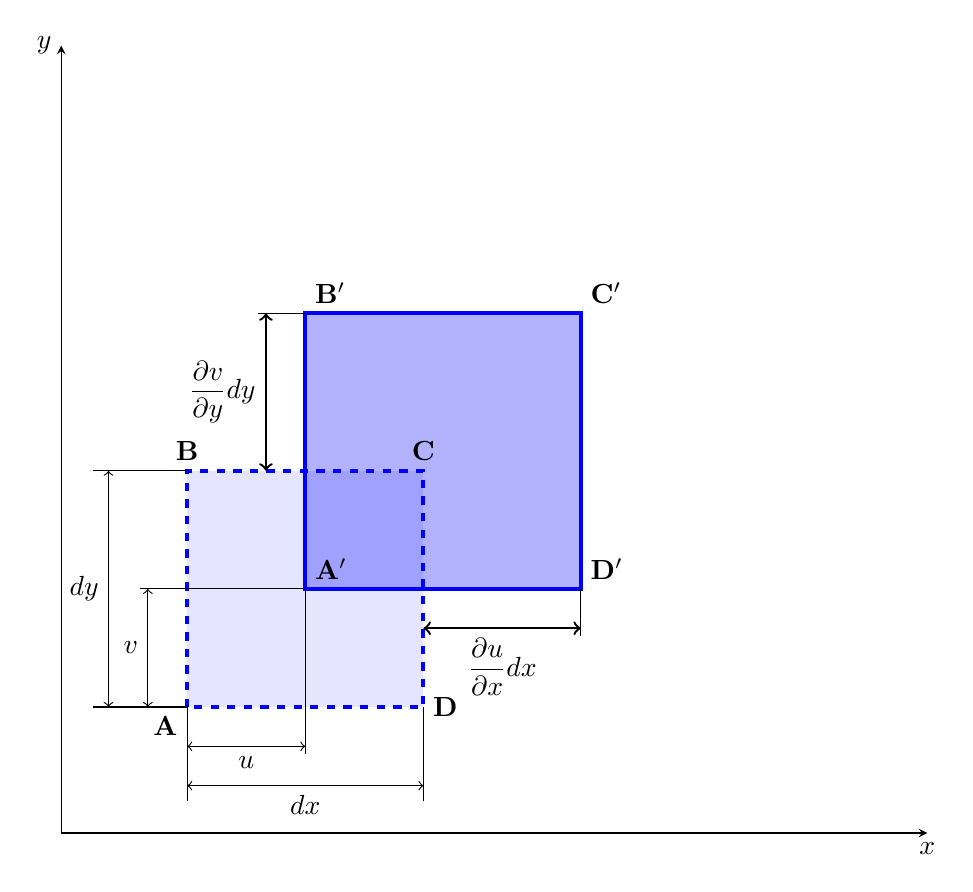
\begin{tikzpicture}
                \draw[-stealth] (0,0) -- (11,0) node[below]{$x$};
                \draw[-stealth] (0,0) -- (0,10) node[left]{$y$};
                \begin{scope}[transform canvas={xshift = 0.6cm, yshift = 0.6cm}]
                    \node (A) at (1,1) {};
                    \node (B) at (1,4) {};
                    \node (C) at (4,4) {};
                    \node (D) at (4,1) {};
                    \draw[line width = 0.5mm, dashed, blue, fill = blue, fill opacity = 0.1] (A.center) -- (B.center) -- (C.center) -- (D.center) -- cycle;
                    
                    
                    \node (A') at (2.5,2.5) {};
                    \node (B') at (2.5,6.0) {};
                    \node (C') at (6,6) {};
                    \node (D') at (6,2.5) {};
                    
        
                    \draw[line width = 0.5mm, blue, fill = blue, fill opacity = 0.3]  (A'.center) -- (B'.center) -- (C'.center) -- (D'.center) -- cycle;
        
                    \draw node[below left] at (A.center) {$\mathbf{A}$};
                    \draw node[above] at (B.center) {$\mathbf{B}$};
                    \draw node[above] at (C.center) {$\mathbf{C}$};
                    \draw node[right] at (D.center) {$\mathbf{D}$};
                    \draw node[above right] at (A'.center) {$\mathbf{A'}$};
                    \draw node[above right] at (B'.center) {$\mathbf{B'}$};
                    \draw node[above right] at (C'.center) {$\mathbf{C'}$};
                    \draw node[above right] at (D'.center) {$\mathbf{D'}$};
        
        
        
        
                    \draw[<->, transform canvas={xshift = -0.5cm}] (A.center)  -- (A'.center -| A.center) node[midway, left]{$v$};
                    \draw[<->, transform canvas={yshift = -0.5cm}] (A.center)  -- (A'.center |- A.center)  node[midway, below]{$u$};
                    
                    \draw[<->, transform canvas={yshift = -1cm}] (A.center)  -- (D.center |- A.center)  node[midway, below]{$dx$};
        
                    \draw[<->, transform canvas={xshift = -1cm}] (A.center)  -- (B.center -| A.center)  node[midway, left]{$dy$};
                    
        
                    \draw (A'.center -| A.center) ++ (-0.6,0) -- (A'.center) -- (A'.center |- A.center) --++ (0,-0.6);
                    \draw ({(-0.2,0)} |- A.center) -- (A.center) -- ({(0,-0.2)} -| A.center);
                    \draw ({(-0.2,0)} |- B.center) -- (B.center);
                    \draw ({(0,-0.2)} -| D.center) -- (D.center);
        
                    \draw[<->,  transform canvas={yshift = -0.5cm}, line width = 0.3mm] (C.center |- A'.center) -- (D'.center) node[midway, below]{$\displaystyle \frac{\partial u}{\partial x} dx$};
                    \draw (D'.center) --++ (0,-0.6);
                    
                    \draw[<->,  transform canvas={xshift = -0.5cm}, line width = 0.3mm] (C.center -| A'.center) -- (B'.center) node[midway, left]{$\displaystyle \frac{\partial v}{\partial y} dy$};
                    \draw (B'.center) --++ (-0.6,0);
        
        
                \end{scope}
            \end{tikzpicture}
        }
        \caption{deformação linear}
        \label{fig:deformacao_elemento_1}
    \end{subfigure}
    \begin{subfigure}[b]{0.45\textwidth}
        \resizebox{\textwidth}{!}{
            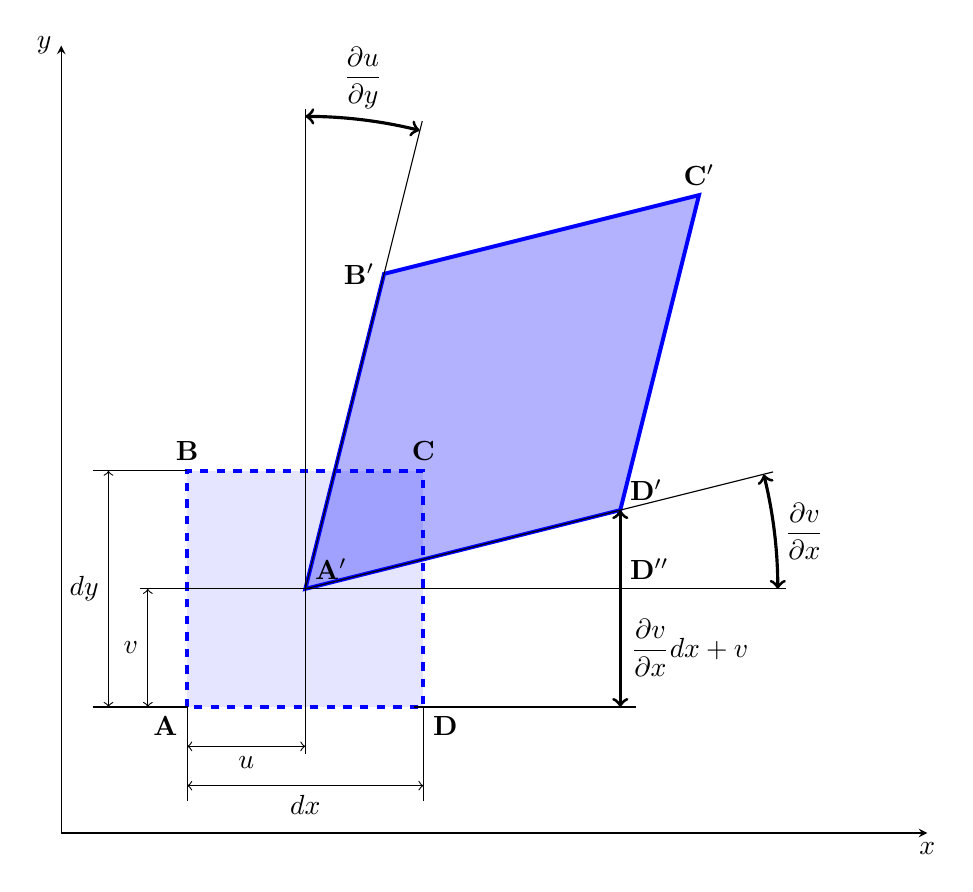
\begin{tikzpicture}
                \draw[-stealth] (0,0) -- (11,0) node[below]{$x$};
                \draw[-stealth] (0,0) -- (0,10) node[left]{$y$};
                \begin{scope}[transform canvas={xshift = 0.6cm, yshift = 0.6cm}]
                    \node (A) at (1,1) {};
                    \node (B) at (1,4) {};
                    \node (C) at (4,4) {};
                    \node (D) at (4,1) {};
                    \draw[line width = 0.5mm, dashed, blue, fill = blue, fill opacity = 0.1] (A.center) -- (B.center) -- (C.center) -- (D.center) -- cycle;
                    
                    
                    \node (A') at (2.5,2.5) {};
                    \node (B') at (3.5,6.5) {};
                    \node (C') at (7.5,7.5) {};
                    \node (D') at (6.5,3.5) {};
                    
        
                    \draw[line width = 0.5mm, blue, fill = blue, fill opacity = 0.3]  (A'.center) -- (B'.center) -- (C'.center) -- (D'.center) -- cycle;
        
                    \draw node[below left] at (A.center) {$\mathbf{A}$};
                    \draw node[above] at (B.center) {$\mathbf{B}$};
                    \draw node[above] at (C.center) {$\mathbf{C}$};
                    \draw node[below right] at (D.center) {$\mathbf{D}$};
                    \draw node[above right] at (A'.center) {$\mathbf{A'}$};
                    \draw node[left] at (B'.center) {$\mathbf{B'}$};
                    \draw node[above] at (C'.center) {$\mathbf{C'}$};
                    \draw node[above right] at (D'.center) {$\mathbf{D'}$};
        
        
                    \draw[<->, transform canvas={xshift = -0.5cm}] (A.center)  -- (A'.center -| A.center) node[midway, left]{$v$};
                    \draw[<->, transform canvas={yshift = -0.5cm}] (A.center)  -- (A'.center |- A.center)  node[midway, below]{$u$};
                    
                    \draw[<->, transform canvas={yshift = -1cm}] (A.center)  -- (D.center |- A.center)  node[midway, below]{$dx$};
        
                    \draw[<->, transform canvas={xshift = -1cm}] (A.center)  -- (B.center -| A.center)  node[midway, left]{$dy$};
                    
        
                    \draw (A'.center -| A.center) ++ (-0.6,0) -- (A'.center) -- (A'.center |- A.center) --++ (0,-0.6);
                    \draw ({(-0.2,0)} |- A.center) -- (A.center) -- ({(0,-0.2)} -| A.center);
                    \draw ({(-0.2,0)} |- B.center) -- (B.center);
                    \draw ({(0,-0.2)} -| D.center) -- (D.center);
        
        
                    
                    \draw (A'.center) -- (A'.center |- C') --++ (0,1.1);
                    \draw (A'.center) -- (A'.center -| C') --++ (1.1,0);
        
                    \draw[shorten >= -2cm] (A'.center) -- (B'.center);
                    \draw[shorten >= -2cm] (A'.center) -- (D'.center);
        
                    \draw[<->, line width = 0.4mm]  (D'.center) -- (D' |- A.center) node[midway, below right]{$\displaystyle \frac{\partial v}{\partial x} dx + v$};
                    \draw (D.west) -- (D -| D') --++ (0.2,0);
        
                    
                    \draw[<->, line width = 0.4mm] (A'.center) ++ (6,0)  arc (0:14:6) node[midway, right]{$\displaystyle \frac{\partial v}{\partial x}$};
        
                    \draw[<->, line width = 0.4mm] (A'.center) ++ (0,6)  arc (90:76:6) node[midway, above]{$\displaystyle \frac{\partial u}{\partial y}$};
        
        
                    \draw (D' |- A') node[above right]{$\mathbf{D''}$};
                \end{scope}
            \end{tikzpicture}
        }
        \caption{deformação angular}
        \label{fig:deformacao_elemento_2}
    \end{subfigure}
    \label{fig:deformacao_elemento}
\end{figure}

O comprimento do segmento antes da deformação $AD$ é o próprio infinitesimal $dx$. Já o comprimento do deformado, é dado pela diferença das posições dos pontos deslocados $||A'D'||$. Em termos do campo de deslocamento, é o mesmo que

\begin{equation}
    ||A'D'|| = (D_x + u(D_x)) - (A_x + u(A_x)),
\end{equation}
em que o subscrito $x$ denota a respectiva componente da posição do ponto.

Como $D_x = A_x + dx$, podemos expandir a função $u$ ao redor de $A_x$, obtendo que\footnote{Os termos $O(3)$ da expansão são desconsiderados pois a diferença entre os pontos é infinitesimal, logo $dx >> dx^2$.}

\begin{equation}
    u(D_x) = u(A_x + dx) = u + \frac{\partial u}{\partial x} dx,
\end{equation}

Portanto,

\begin{equation}
    ||A'D'|| - ||AD|| = (D_x + u + \frac{\partial u}{\partial x} dx - u - A_x) - (D_x - A_x) = \frac{\partial u}{\partial x} dx
\end{equation}
em que $A_x$ representa a projeção do ponto $A$ em $x$.
Agora, substituindo essa expressão na equação \ref{eq:deforma}, temos a definição da deformação normal na direção de $x$, em que
\begin{equation}
    \epsilon_x = \frac{\partial u}{\partial x}.
\end{equation}
O mesmo procedimento pode ser feito tanto na direção de $y$, com o segmento $AB$,quanto na direção de $z$, assumindo um elemento infinitesimal cúbico, tal qual a figura \ref{fig:estado_de_tensao} do estado de tensão, obtendo-se, assim, todas as definições básicas de deformação normal \cite{popov}:

\begin{equation}
    \epsilon_x = \frac{\partial u}{\partial x}, \qquad \epsilon_y = \frac{\partial u}{\partial y}, \qquad \epsilon_z = \frac{\partial u}{\partial z}. \\
\end{equation}  

Na figura \ref{fig:deformacao_elemento_2}, ocorre a deformação por cisalhamento, em que os segmentos $AD$ e $AB$ são, além de transladados, rotacionados em torno de $A'$, de modo a distorcer a geometria do elemento. Agora, a deformação ocorre tanto na direção em $x$, quanto em $y$, e é definida pela alteração do ângulo reto $\angle BAD$, determinada, em termos do campo de deslocamentos (tal como na deformação normal) analisando o triângulo $A'D'D''$.

A função $v$, quando variada em $x$ da posição de $A$ até $D$, descreve o deslocamento dos pontos da face inferior do elemento infinitesimal na direção de $y$, ou seja, a hipotenusa do triângulo $A'D'D''$. A inclinação, portanto, dessa reta é própria derivada de $v$ na direção $x$, ou seja,

\begin{equation}
    \angle D'A'D'' = \tan{\frac{\partial v}{\partial x}} \approx \frac{\partial v}{\partial x}.\footnotemark
\end{equation}\footnotetext{É essa aproximação é devida pois para ângulos suficientemente pequenos: $\tan \theta = \theta$, o que pode ser verificado expandindo a série de Taylor ao redor de $x=0$.}

Outro modo de se obter a mesma expressão é aplicar a definição trigonométrica da tangente sobre o triângulo $A'D'D''$, de forma que, em suma,

\begin{align}
    |A'D''|             &= \sqrt{dx^2 -  \left(\frac{\partial v}{\partial x}dx\right)^2}, \text{Teorema de Pitágoras}\\
                         &= \sqrt{dx^2}, \left(\frac{\partial v}{\partial x}dx\right)^2 << dx,\\
    |A'D''|              &= dx,\\
    \tan{\angle D'A'D''} &= \frac{|D'D''|}{|A'D''|}, \\
                         &= \frac{\partial v}{\partial x}dx \frac{1}{dx},\\
                         & = \frac{\partial v}{\partial x}.\\
\end{align}
O mesmo pode ser feito na direção de $y$, para encontrar a inclinação do segmento $A'B'$, como também para $z$, considerando um elemento infinitesimal cúbico.

Portanto, a deformação cisalhante do elemento infinitesimal é dada, em termos do deslocamento, por
\begin{gather}
        \gamma_{xy} = \gamma_{yx} = \frac{\partial u}{\partial y} + \frac{\partial v}{\partial x} \\
        \gamma_{xz} = \gamma_{zx} = \frac{\partial w}{\partial x} + \frac{\partial u}{\partial z} \\
        \gamma_{yz} = \gamma_{zy} = \frac{\partial w}{\partial y} + \frac{\partial v}{\partial z} \\
\end{gather}
Por convenção\footnote{Essa convenção não é mero simbolismo, mas faz com que o tensor de deformações tenha propriedades interessantes, como a possibilidade de se descrever a energia interna em termos do produto escalar entre os tensores de deformação e de tensão na notação de Voigt.} 

O tensor de deformações é
\begin{gather}
    [\mathbf{\epsilon}] = 
    \begin{bmatrix}
        \varepsilon_{xx} & \varepsilon_{xy} & \varepsilon_{xz} \\
        \varepsilon_{yx} & \varepsilon_{yy} & \varepsilon_{yz} \\
        \varepsilon_{zx} & \varepsilon_{zy} & \varepsilon_{zz} \\
    \end{bmatrix}
        =
    \begin{bmatrix}
        \frac{\partial u}{\partial x} & \frac{1}{2} \left(\frac{\partial u}{\partial y}+\frac{\partial v}{\partial x}\right) & \frac{1}{2} \left(\frac{\partial u}{\partial z}+\frac{\partial w}{\partial x}\right) \\
        \frac{1}{2} \left(\frac{\partial v}{\partial x}+\frac{\partial u}{\partial y}\right) & \frac{\partial v}{\partial y} & \frac{1}{2} \left(\frac{\partial v}{\partial z}+\frac{\partial w}{\partial y}\right) \\
        \frac{1}{2} \left(\frac{\partial w}{\partial x}+\frac{\partial u}{\partial z}\right) & \frac{1}{2} \left(\frac{\partial w}{\partial y}+\frac{\partial v}{\partial z}\right) & \frac{\partial w}{\partial z} \\
    \end{bmatrix}.
    \label{eq:tensor_de_deformacoes}
\end{gather}

Tal como o tensor de tensões, o tensor de deformações é simétrico, e, portanto, só possui seis componentes independentes. Na notação de Voigt, de acordo com \citeshort{roylance},
\begin{equation}
    \{\epsilon\} = \begin{bmatrix}
        \epsilon_x & \epsilon_y & \epsilon_z & \gamma_{xy} & \gamma_{xz} & \gamma_{yz}
    \end{bmatrix}^t
\end{equation}

\section{A Lei de Hooke}

Em corpos sólidos, a deformação está relacionada diretamente com a tensão em seu interior, de modo que se possa, dentro de certas condições, descrever uma transformação linear entre elas. Essa transformação é nomeada \emph{Lei de Hooke}, e, utilizando a notação de Voigt, é descrita por

\begin{equation}
    \{\sigma\} = [\bm{C}] \{\epsilon\}.
    \label{eq:lei_de_hooke}
\end{equation}
em que $[\bm{C}]$ é denominada \emph{matriz constitutiva}\footnote{A matriz constitutiva é uma forma de notação abreviada para descrever essa relação. Da mesma forma que o tensor de tensões é abreviado por uma matrix coluna na notação de Voigt, devido a sua simetria, a matriz constitutiva é a abreviação de do tensor de elasticidade, um tensor de quarta ordem que mapeia o espaço das deformações no das tensões.}, e é definida em termos das características do material do corpo, tais como módulo de elasticidade e coeficiente de Poisson. 

\subsection{A Lei de Hooke Uniaxial}

Sejam o quadrilátero $\mathcal{B}$, um corpo sólido, homogêneo, em equilíbrio, de comprimento $L$, engastado em sua face esquerda, e de seção transversal $A$. Seja também $F$, uma força constante que atua sobre a face direita de $\mathcal{B}$, na direção de $x$, que a deforma em $\mathcal{B}'$ até um comprimento $L+\Delta L$, tal como na figura \ref{fig:barra_deformada_1}. 

A tensão desenvolvida em um ponto, suficientemente longe da região de aplicação da carga, de uma seção $S$ de $\mathcal{B}$, perpendicular à força $\vec{F}$, pode ser descrita em termos do módulo de elasticidade, $E$ (também denominado módulo de Young), que é uma característica intrínseca do material de $\mathcal{B}$, e da deformação, $\epsilon_x$, atuando na mesma direção da força. Essa relação, denominada \emph{Lei de Hooke Uniaxial}, é linear da forma
\begin{equation}
    \sigma_x = E \epsilon_x.
    \label{eq:lei_de_hooke_uniaxial}
\end{equation} 
A unidade de $E$ é a mesma de $\sigma_x$, o que é coerente, pois $\epsilon_x$ é adimensional, ou seja, o módulo de elasticidade é medido, no SI, em Pascal.

\begin{figure}
    \centering
    \caption{Barra deformada}
    \begin{subfigure}[b]{\textwidth}
        \resizebox{\textwidth}{!}{
            \begin{tikzpicture}[
                    marrow/.style = {arrows = {-Latex[width=8pt, length=10pt]}}
                ]
                
                \draw[->] (0,0) --++ (0,3) node[above]{$y$};
                \draw[->] (0,0) --++ (10,0) node[above]{$x$};

                \draw[thick, blue, fill = blue, fill opacity = 0.3] (0,0) rectangle (8,2);
                \draw (4,1) node{$\bm{B}$};
                
                \draw[thick, blue, fill = blue, fill opacity = 0.3, dashed] (0,0.2) rectangle (8.5,1.8);

                \draw[|<->|] (0,2.1) --++ (8,0) node[above, midway]{$L$};
                \draw[|<->|] (8,2.1) --++ (0.5,0) node[above,midway]{$\Delta L$};

                \draw[marrow] (8.5,1) --++ (2,0) node[right]{$\vec{F}$};
                
            \end{tikzpicture}
        }
        \caption{por tração}
        \label{fig:barra_deformada_1}
    \end{subfigure}
    \begin{subfigure}[b]{\textwidth}
        \resizebox{\textwidth}{!}{
            \begin{tikzpicture}[
                marrow/.style = {arrows = {-Latex[width=4pt, length=10pt]}, line width = 0.5mm}
            ]

            \draw[->] (0,0) --++ (0,3) node[above]{$y$};
            \draw[->] (0,0) --++ (10,0) node[above]{$x$};
            \draw[thick] (8,2)-- (8,3.10) (8,0) -- (8.5,2) --++ (0.25, 1);
            \draw[thick, blue, fill = blue, fill opacity = 0.3, dashed] (0,0) rectangle (8,2);


            \draw[thick, red, fill = red, fill opacity = 0.3] (0,0) -- (0.5,2) -- (8.5,2) -- (8,0) -- cycle;

            \draw[|<->|] (0,2.1) --++ (8,0) node[above, midway]{$L$};
            \foreach \n in {0,1,...,7}{
                \draw[marrow] ({\n},2) --++ (1.05,0);
            }

            \draw (1,2) |- (2,3) node[right]{$Q$};
            \draw (4,1) node{$\bm{B}$};

            \draw[<->] (8,2.7) arc (90:71:2) node[midway, above]{$\gamma$}	;
            \end{tikzpicture}
        }
        \caption{por cisalhamento}
        \label{fig:barra_deformada_2}
    \end{subfigure}
\end{figure}

Essa relação desconsidera outros efeitos de deformação no interior do sólido, como a deformação transversal, $\epsilon_y$ (que pode ser observada como o encurtamento da altura da barra na figura \ref{fig:barra_deformada_1}), e a por cisalhamento, $\gamma_{xy}$. \footnote{O limite de elasticidade do material é determinado experimentalmente, observando como se deforma sobre carregamentos controlados, determinando a região de deformações em que o material preserva-se na Lei de Hooke, ou seja, mantém uma relação linear entre deformação e tensão, e ao ser aliviado dos carregamentos externos, volta à geometria original.}.

\subsection{A Lei de Hooke em Cisalhamento}

Seja um quadrilátero $\mathcal{B}$, um corpo sólido, homogêneo, em equilíbrio, de comprimento $L$, engastado em sua face inferior, e de seção transversal $S$, e seja $Q$, uma carregamento constante que atua sobre a face superior de $\mathcal{B}$, tangencialmente, na direção de $x$, que a deforma em $\mathcal{B}'$, inclinando-a, até um ângulo $\gamma$, tal como na figura \ref{fig:barra_deformada_2}. 

A tensão desenvolvida em uma seção $S$ de $\mathcal{B}$, paralela ao carregamento de  $Q$, pode ser descrita em termos do módulo de cisalhamento, $G$, que é uma característica intrínseca do material de $\mathcal{B}$, e da deformação angular, $\gamma$, atuando na inclinação das seções verticais. Essa relação, denominada \emph{Lei de Hooke em Cisalhamento}, é linear da forma

\begin{equation}
    \tau_{xy} = G \gamma_{xy} \implies \tau_{xy} = 2G \epsilon_{xy}.
    \label{eq:lei_de_hooke_cisalhamento}
\end{equation}
O módulo de cisalhamento tem a mesma unidade de tensão, e, assim como o módulo de Young ($\gamma$ é adimensional), não depende da geometria do corpo, mas do material de que é feito.

\subsection{O Coeficiente de Poisson}

Na deformação uniaxial de um corpo sólido, tal como na figura \ref{fig:barra_deformada_1}, é razoável que o corpo também se deforme nas direções transversais, de forma que existe, dentro de determinados limites do regime elástico, uma relação entre essa deformações. Observa-se, por meio da experiência prática, que a deformação transversal geralmente é negativa, o corpo tende a se contrair quando submetido a uma deformação axial positiva. Se o corpo se deforma ao longo de $x$ um $\epsilon_x > 0$, ele se contrai em $y$, ou seja, desenvolve uma deformação $\epsilon_y < 0$, de forma que, de acordo com \citeshort{lub}, para deformação axial
\begin{equation}
    \nu = -\frac{\epsilon_y}{\epsilon_x},
    \label{eq:coeficiente_de_poisson}
\end{equation}
em que $\nu$ representa o coeficiente de Poisson, a razão entre a deformação transversal e a deformação axial.

O coeficiente de Poisson é uma característica intrínseca do material, e, assim como os módulos de Young e de cisalhamento, não depende da geometria do corpo, mas do material de que é feito (dentre outras condições mais específicas), entretanto, pode variar conforme a direção da deformação, para materiais que não são isotrópicos, diferentemente, de $\mathcal{B}$. Aqui $\nu$ é tratado como constante.

\subsection{O Princípio da Sobreposição \& A Lei de Hooke Generalizada}

\begin{citacao}
    O \emph{princípio da sobreposição} permite a aditividade de efeitos (leia-se, deformações) na presença de múltiplas causa (leia-se, tensões). Invocando esse princípio, nós podemos expressão o total de deformação percebida pelo corpo como a soma de todas as deformações devidas aos componentes individuais de tensão presentes no corpo. \cite[pág. 252, tradução livre]{lub}
\end{citacao}

Esse princípio é válido quando, de acordo com \cite{lub}:
\begin{enumerate}
    \item as equações de equilíbrio são lineares nas tensões;
        
    Observando a equação \ref{eq:equilibrio_governo}, é possível notar que, dado dois conjuntos de tensões que satisfazem as equações de equilíbrio, a soma desses dois conjuntos também o faz, ou seja, as equações de equilíbrio são lineares nas tensões. Em termos matemáticos, é o mesmo que demonstrar a linearidade do operador divergência ($\nabla \cdot (*)$).
    \item as relações entre deformação e deslocamento são lineares;
        
    Tal como no item anterior, é possível demonstrar essa propriedade tomando dos conjuntos de deslocamentos arbitrários, que, quando somados, levam um conjunto de deformações que equivale ao somatório das deformações de cada conjunto de deslocamentos individualmente.
    \item as relações entre tensão e deformação são lineares.
        
    Observando as relações definidas para o módulo de Young, o módulo de cisalhamento e o coeficiente de Poisson, fica evidente que todas são lineares.
\end{enumerate}

Assumindo agora que sobre um elemento infinitesimal cúbico, tal qual a figura \ref{fig:estado_de_tensao}, atuam todas as componentes do tensor de tensões, de modo que, utilizando as relações entre deformação e tensão, das equações \ref{eq:lei_de_hooke_uniaxial} e \ref{eq:lei_de_hooke_cisalhamento}, como também a relação entre deformações, equação \ref{eq:coeficiente_de_poisson}, é possível determinar o efeito de deformação causado por cada componente de tensão, tal que, devido à tensão $\sigma_x$, o elemento infinitesimal percebe as deformações

\begin{equation}
    \epsilon_x =\frac{\sigma_x}{E}, \qquad \epsilon_y = -\nu \frac{\sigma_x}{E}, \qquad \epsilon_z = -\nu \frac{\sigma_x}{E}.
\end{equation}
As outras tensões, $\sigma_y$ e $\sigma_z$, se comportam de forma análoga, de modo que
\begin{gather}
    \epsilon_x =-\nu \frac{\sigma_y}{E}, \qquad \epsilon_y = \frac{\sigma_y}{E}, \qquad \epsilon_z = -\nu \frac{\sigma_y}{E}, 
\end{gather}
\begin{gather}
    \epsilon_x =-\nu \frac{\sigma_z}{E}, \qquad \epsilon_y = -\nu \frac{\sigma_z}{E}, \qquad \epsilon_z = \frac{\sigma_z}{E}.
\end{gather}

As tensões de cisalhamento, $\tau_{xy}$, $\tau_{xz}$ e $\tau_{yz}$, por sua vez, causam as deformações angulares,
\begin{gather}
    \gamma_{xy} = \frac{\tau_{xy}}, \qquad \gamma_{xz} = \frac{\tau_{xz}}{G}, \qquad \gamma_{yz} = \frac{\tau_{yz}}{G}.
\end{gather}

Sobrepondo as deformações axiais para cada eixo, e as deformações angulares, é possível determinar as relaçãoes entre todas as tensões e todas as deformações, denominada \emph{lei de Hooke generalizada}:
\begin{gather}
    \epsilon_x = \frac{\sigma_x}{E} - \nu \frac{\sigma_y}{E} - \nu \frac{\sigma_z}{E}, \\
    \epsilon_y = -\nu \frac{\sigma_x}{E} + \frac{\sigma_y}{E} - \nu \frac{\sigma_z}{E}, \\
    \epsilon_z = -\nu \frac{\sigma_x}{E} - \nu \frac{\sigma_y}{E} + \frac{\sigma_z}{E}, \\
    \gamma_{xy} = \frac{\tau_{xy}}{G}, \\ 
    \gamma_{xz} = \frac{\tau_{xz}}{G}, \\
    \gamma_{yz} = \frac{\tau_{yz}}{G}.
    \label{eq:lei_de_hooke_generalizada}
\end{gather}
O módulo de cisalhamento pode ser determinado em termos da razão de Poisson e do módulo de Young, de modo que\footnote{A demonstração dessa relação se utiliza daas fórmulas de rotação dos tensores de deformações e de tensores, que não são tratadas aqui.}
\begin{gather}
    G = \frac{E}{2(1+\nu)}.
\end{gather}

Utilizando a notação de Voigt, a Lei de Hooke generalizada pode ser em forma compacta como

\begin{equation}
    \begin{Bmatrix}
        \epsilon_x \\
        \epsilon_y \\
        \epsilon_z \\
        \gamma_{xy} \\
        \gamma_{xz} \\
        \gamma_{yz}
    \end{Bmatrix}
    =
    \frac{1}{E}
    \begin{bmatrix}
        1 & -\nu & -\nu & 0 & 0 & 0 \\
        -\nu & 1 & -\nu & 0 & 0 & 0 \\
        -\nu & -\nu & 1 & 0 & 0 & 0 \\
        0 & 0 & 0 & 2(1+\nu) & 0 & 0 \\
        0 & 0 & 0 & 0 & 2(1+\nu) & 0 \\
        0 & 0 & 0 & 0 & 0 & 2(1+\nu)
    \end{bmatrix}
    \begin{Bmatrix}
        \sigma_x \\
        \sigma_y \\
        \sigma_z \\
        \tau_{xy} \\
        \tau_{xz} \\
        \tau_{yz}
    \end{Bmatrix},
    \label{eq:lei_de_hooke_generalizada_matricial}
\end{equation}

Invertendo esse sistema, obtemos a matriz constitutiva da equação \ref{eq:lei_de_hooke},

\begin{equation}
    \{\sigma\} = \underbrace{\frac{E}{(1+\nu)(1-2\nu)}
    \begin{bmatrix} 1-\nu & \nu & \nu & 0 & 0 & 0 \\
        \nu & 1-\nu & \nu & 0 & 0 & 0 \\
        \nu & \nu & 1-\nu & 0 & 0 & 0 \\
        0 & 0 & 0 & \frac{1-2\nu}{2} & 0 & 0 \\
        0 & 0 & 0 & 0 & \frac{1-2\nu}{2} & 0 \\
        0 & 0 & 0 & 0 & 0 & \frac{1-2\nu}{2} 
    \end{bmatrix}}_{[\bm{C}]}
    \{\epsilon\}
\end{equation}
Para que essa matriz exista, é necessário que $-1 < \nu < \frac{1}{2}$.\footnote{Materiais com $\nu = 0.5$ são chamados de incompressíveis, pois não sofrem deformações volumétricas.}

\subsection{Estado Plano de Deformação e de Tensão}


Quando se analisa um problema plano, é possível simplificar as relações descritas pela matriz $[\bm{C}]$ em dois casos, observando a rigidez do corpo nas direção transversal ao plano de análise.

O Estado Plano de Tensão (EPT) ocorre quando a rigidez do corpo na direção transversal é muito baixa (como uma chapa ou uma placa), fazendo com que a tensão nessa direção possa ser neglicenciada, ou seja, $\sigma_z = \tau_{xz} = \tau_{yz} = 0$. Nesse caso, a lei de Hooke generalizada se reduz a, \footnote{Tanto a matriz constitutiva do EPT e quando do EPD são facilmente deduzidas da lei de Hooke generalizada, apenas atribuindo os valores nulos e trabalhando com as inversas da matriz $[\bm{C}]$.}

\begin{gather}
    \begin{Bmatrix}
        \epsilon_x \\
        \epsilon_y \\
        \gamma_{xy}
    \end{Bmatrix} = \frac{1}{E} \begin{bmatrix}
        1 & -\nu & 0 \\
        -\nu & 1 & 0 \\
        0 & 0 & (1+\nu)
    \end{bmatrix}
    \begin{Bmatrix}
        \sigma_x \\
        \sigma_y \\
        \tau_{xy}
    \end{Bmatrix}, \\
    \epsilon_z = -\nu \frac{\sigma_x}{E} - \nu \frac{\sigma_y}{E}.
\end{gather}
$\epsilon_z$ passou a ser uma variável dependente, pois é determinada, totalmente, pelas outras deformações. \cite[pág. 90]{Zin}

As Relações que definem a matriz constitutiva para o estado plano de tensão:

\begin{gather}
    \begin{Bmatrix}
        \sigma_x \\
        \sigma_y \\
        \tau_{xy}
    \end{Bmatrix} = \frac{E}{1-\nu^2} 
    \underbrace{\begin{bmatrix}
        1 & \nu & 0 \\
        \nu & 1 & 0 \\
        0 & 0 & \frac{1-\nu}{2}
    \end{bmatrix}}_{[\bm{C}]}
    \begin{Bmatrix}
        \epsilon_x \\
        \epsilon_y \\
        \epsilon_{xy}
    \end{Bmatrix}.
\end{gather}

O Estado de Plano de Deformação (EPD), por sua vez, ocorre quando o corpo é muito rígido na direção transversal (como uma barragem ou um muro), fazendo com que a deformação nessa direção possa ser neglicenciada, ou seja, $\epsilon_z = \gamma_{xz} = \gamma_{yz} = 0$. Nesse caso, a lei de Hooke generalizada se reduz a

\begin{gather}
    \begin{Bmatrix}
        \sigma_x \\
        \sigma_y \\
        \tau_{xy}
    \end{Bmatrix} = \frac{E}{(1+\nu)(1-2\nu)} 
    \underbrace{\begin{bmatrix}
        1 - \nu & \nu & 0 \\
        \nu & 1 - \nu & 0 \\
        0 & 0 & \frac{1-2\nu}{2}
    \end{bmatrix}}_{[\bm{C}]}
    \begin{Bmatrix}
        \epsilon_x \\
        \epsilon_y \\
        \gamma_{xy}
    \end{Bmatrix}, \\
    \sigma{z} = \nu (\sigma_x + \sigma_y)
\end{gather}
$\gamma_{xz}$ passou a ser uma variável dependente, pois é determinada, totalmente, pelas outras deformações.  \cite[pág. 91]{Zin}

\section{Teoria da Energia de Distorção Máxima: A Tensão Equivalente de Von Mises}

A Teoria da Energia de Distorção máxima propõe que:
\begin{citacao}
    o escoamento em um material dúctil ocorre quando a energia de distorção por unidade de volume do material ultrapassa a energia de distorção por unidade de volume do mesmo material quando submetido a escoamento em um ensaio de tração simples. \cite{Hibbeler}
\end{citacao}

Essa proposição surge da observação que materiais dúcteis sob carregamentos hidrostáticos exibem uma resistência muito maior que em simples ensaios de tração uniaxial, e que, portanto, o escoamento não é um fenômeno compreendido, simplesmente, pela tração ou compressão, mas, majoritariamente, pela distorção do material. \cite{Hibbeler}

A energia por unidade de volume, devida à deformação do material, é definida por um produto da tensão pela deformação. Em um elemento orientado sob tensões principais, de acordo com \cite{Hibbeler}
\begin{equation}
    \mathcal{U} = \frac{1}{2} (\sigma_1 \epsilon_1 + \sigma_2 \epsilon_2 + \sigma_3 \epsilon_3),
\end{equation}
em que $\mathcal{U}$ denota a energia por unidade de volume, $\sigma_i$ as tensões principais.

Substituindo as deformações pelas tensões, utilizando a lei de Hooke generalizada, equação \ref{eq:lei_de_hooke_generalizada}, temos que

\begin{equation}
    \mathcal{U} = \frac{1}{2E} \left[ \sigma_1^2 + \sigma_2^2 + \sigma_3^2 - 2\nu(\sigma_1\sigma_2 + \sigma_1\sigma_3 + \sigma_2 \sigma_3) \right].
    \label{eq:energia_deformacao}
\end{equation}

Essa energia pode sem compreendia como a soma de duas parcelas: a energia de deformação volumétrica, $u_v$, e a energia de deformação por cisalhamento, $u_d$. A energia de deformação volumétrica é a energia de deformação que tende a alterar o volume do elemento, sem distorcer sua geometria, ou seja, a energia de deformação devido à tensão média das tesões principais. Substituindo, então, as tensões principais pela tensão média na equação anterior, temos que
\begin{equation}
    \mathcal{U}_v = \frac{3\bar{\sigma}^2}{2E} (1 - 2\nu),
    \label{eq:energia_deformacao_volumetrica}
\end{equation}
em que $\bar{\sigma} = \frac{1}{3} (\sigma_1 + \sigma_2 + \sigma_3)$ é a tensão média. 

A energia de distorção, portanto, é a diferença entre a energia total e a energia volumétrica, de modo que

\begin{equation}
    \mathcal{U}_d = \mathcal{U} - \mathcal{U}_v = \frac{1 +\nu}{3E} \left[\frac{(\sigma_1 - \sigma_2)^2 + (\sigma_2 - \sigma_3)^2 + (\sigma_3 - \sigma_1)^2}{2} \right].
    \label{eq:energia_deformacao_distorcao}    
\end{equation}

Fazendo $\sigma_2 = \sigma_3 = 0$, temos a energia de deformação para o caso de tração uniaxial, de modo que
\begin{equation}
    \mathcal{U} = \frac{1 + \nu}{3}\sigma_e^2,
\end{equation}
em que $\sigma_e$ é a tensão admissível do material num ensaio de tração. \cite{Hibbeler}

Portanto, de acordo com o princípio da energia de distorção máxima, o escoamento ocorre quando a energia de distorção ultrapassa a energia de distorção de um ensaio de tração simples, ou seja, quando \cite{Hibbeler}

\begin{equation}
    \sigma_e \leq \left[\frac{(\sigma_1 - \sigma_2)^2 + (\sigma_2 - \sigma_3)^2 + (\sigma_3 - \sigma_1)^2}{2} \right]^{1/2}.
\end{equation}

O lado direito dessa inequação pode ser interpretado como uma tensão equivalente ou efetiva do estado de tensão dado pelas tensões principais. De acordo com \cite{Hibbeler}, essa tensão é denominada \emph{tensão equivalente de von Mises}, definida por

\begin{equation}
    \sigma_{eq} = \left[\frac{(\sigma_1 - \sigma_2)^2 + (\sigma_2 - \sigma_3)^2 + (\sigma_3 - \sigma_1)^2}{2} \right]^{1/2}.
    \label{eq:tensao_equivalente_von_mises}
\end{equation}

Em termos de um sistema $xyz$, e utilizando todas as componentes do tensor de tensões, a tensão equivalente de von Mises pode ser expressa por 

\begin{equation}
    \sigma_{eq} = \frac{1}{\sqrt{2}} \left[ (\sigma_x - \sigma_y)^2 + (\sigma_y - \sigma_z)^2 + (\sigma_z - \sigma_x)^2 + 6(\tau_{xy}^2 + \tau_{yz}^2 + \tau_{zx}^2)\right].
    \label{eq:tensao_equivalente_von_mises_xyz}
\end{equation}